\documentclass[a4paper,12pt]{article} 


\usepackage[T2A]{fontenc}			% кодировка
\usepackage[utf8]{inputenc}			% кодировка исходного текста
\usepackage[english,russian]{babel}	% локализация и переносы


% Математика
\usepackage{amsmath,amsfonts,amssymb,amsthm,mathtools} 

\usepackage{gensymb}	
\usepackage{wasysym}

% Картинки
\usepackage{graphicx}
\graphicspath{{images/}}

%Заговолок
\usepackage[left=2cm,right=2cm,
    top=1cm,bottom=1cm,bindingoffset=0cm]{geometry}

\usepackage{titling}


\author{Петров Артём Антонович, группа 721}
\title{"Лабораторная работа № 2.3.1 ""}
\date{\today}

\begin{document} % начало документа

\begin{minipage}[t][5cm]{\textwidth}
\maketitle
\end{minipage}


\textbf{Цель работы:} 1) (техническая) измерение объёмов форвакуумной и высоковакуумной частей установки. 2) определение скорости откачки системы в разных режимах.
\bigskip

\textbf{Оборудование:} вакуумная установка.
\bigskip

\textbf{Теория:}
\bigskip

Рассмотрим процесс откачки.

Производительность насоса определяется скоростью откачки W (л/с): объёмом газа, удаляемым из сосуда за единицу времени при постоянном давлении $P$. Основное уравнение, описывающее процесс откачки:

\begin{equation}\label{eq-basic}
-VdP = (PW - Q_d - Q_p - Q_o)dt
\end{equation}

Где $Q_d$ - кл-во газа, десорбирующегося с поверхности сосудов, $Q_p$ - кол-во газа поступающее назад из насоса, $Q_o$ - кол-во газа, поступающего из внешней среды. Q измеряется в величинах PV (домножением на RT/$\mu$ получим массу газа). Видно, что процесс откачки системы зависит не только от W.

При установившемся предельном давлении $P_{lim}$ получим: 
\[\frac{dP}{dt} = 0\]

откуда, 

\begin{equation}\label{eq-lim}
P_{lim}W = Q_d + Q_p + Q_o
\end{equation}

\[W = \frac{\sum Q_i}{p_{lim}}\]

Считая W, $Q_d$, $Q_p$ и $Q_o$ постоянными, проинтегрируем \ref{eq-basic} используя \ref{eq-lim}:

\begin{equation}
P - P_{lim} = (P_0 - P_{lim})\exp(-\frac{W}{V}t)
\end{equation}

$\tau = V/W$ - постоянная времени откачки. Она является показателем эффективности откачки всей системы.  

Рассмотрим теперь, от чего зависит скорость откачки системы. Математическое описание такой системы схоже с законами Кирхгофа для электрических цепей. 

Из теории известно следующее соотношение при последовательном соединении элементов:

\begin{equation}\label{eq-resist}
\frac{1}{W} = \frac{1}{W_p} + \frac{1}{C_1} + \frac{1}{C_2} + ... 
\end{equation}

где W - скорость откачки системы, $W_p$ - скорость откачки собственно насоса, $C_1$, $C_2$, ... - пропускные способности элементов системы.

Из \ref{eq-resist} видно, что эффективность откачки значительно зависит не только от параметров насоса, но и от параметров труб и клапанов.

Рассмотрим течение газа через трубу. Характер течения газа существенно зависит от соотношения между размерами системы и длиной свободного пробега молекул.

Для количества газа, протекающего через трубу в условиях высокого вакуума (в кнудсеновском режиме) справедлива формула:

\begin{equation}\label{eq-flowing}
\frac{d(PV)}{dt} = \frac{4}{3} r^3 \sqrt{\frac{2\pi RT}{\mu}} \frac{P_2-P_1}{L}
\end{equation}

где $P_1$ и $P_2$ - давление на концах трубы, r - радиус трубы, L - длина трубы.

Приняв $P_1$ равным нулю, получим для газа покидающего установку при давлении $P = P_2$ такую формулу:

\begin{equation}\label{eq-tube-resist}
C_t = \frac{4}{3} \frac{r^3}{L}\sqrt{\frac{2\pi RT}{\mu}} 
\end{equation}

где $C_t$ - пропускная способность трубы. Также при расчёте вакуумных установок полезной является необходимым учитывать пропускную способность отверстий (например, кранов). Для них есть формула:

\begin{equation}\label{eq-hole}
\nu = \frac{1}{4}Sn\overline{v}
\end{equation}

где $\nu$ — число молекул, вылетающих из отверстия в вакуум в единицу
времени, $S$ — площадь отверстия, $n$ — концентрация молекул перед отверстием, $\overline{v}$ — средняя скорость молекул газа.

Подставляя $\nu = dN/dt$, $N = PV/kT$, $n = p/kT$ в \ref{eq-hole} получим для газа, покидающего установку через отверстие при постоянном давлении P:

\begin{equation}\label{eq-hole-resist}
C_h = (\frac{dV}{dt})_h = S\frac{\overline{v}}{4} 
\end{equation}

где $C_h$ - пропускная способность отверстия.

Для диффузионного насоса можно считать, что все молекулы, прошедшие через входное отверстие будут затянуты струёй пара, а значит для него $W_p$ будет равна $C_h$ отверстия, с площадью, равной площади кольцевого зазора на входе в диффузионный насос, с одной стороны которого откачиваемый газ, а с другой - пустота.

\bigskip

\textbf{Установка:}
\medskip

\begin{figure}[ht]
\centering
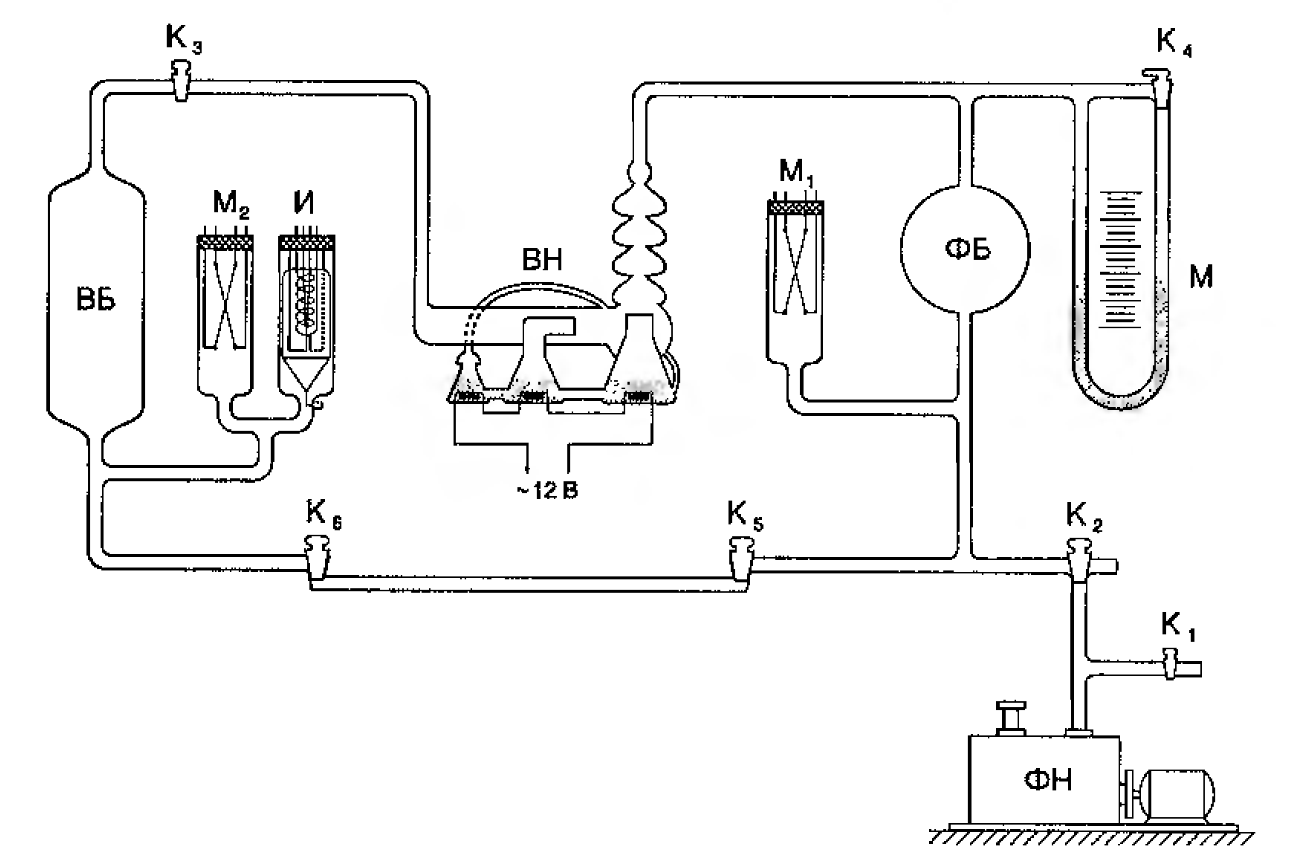
\includegraphics[width=170mm]{schema.png}
\caption{Схема установки: ФН - форвакуумный насос, ФБ - ворвакуумный объём, ВН - высоковакуумный насос, ВБ - высоковакуумный объём, $M_1, M_2, M, \text{И}$ - два термопарных, масляной и ионный манометры соответственно, $K_1 - K_6$ - краны. Между кранами $K_5$ и $K_6$ расположен капилляр. $K_3$ отделяет высоковакуумную часть установки от форвакуумной. $K_4$ служит для "включения"  масляного манометра. $K_1$ и $K_2$ обеспечивают работу форвакуумного насоса.}\label{schema}
\end{figure}

Схема установки показана на рис. \ref{schema}.

Устройство используемых манометров и вакуумных насосов полагается общеизвестным и не требующим детального рассмотрения в рамках этой работы.

\bigskip

\textbf{Ход работы:}
\bigskip

\textbf{1) определение объёмов частей установки:}

1) Напустим атмосферу в установку.

2) Запрём немного воздуха при атмосферном давлении между кранами $K_5$ и $K_6$.

3) Откачаем установку форвакуумным насосом

4) Отключим насос и подготовим масляной манометр к измерениям.

5) Выпустим запертый воздух в форвакуумную часть установки. По закону Бойля-Мариотта вычислим объём форвакуумной части. Зная изначальные давление и объём запертого воздуха.

6) Соединим высоковакуумную часть с форвакуумной. По закону Бойля-Мариотта вычислим объём высоковакуумной части.

7) Повторим измерения ещё раз.

\textbf{2) определение скорости откачки:}

1) Откачаем установку до высокого вакуума согласно инструкции и запишем значение $P_{lim}$.

2)Найдём скорость откачки по улучшению вакуума во время откачки. (Снимем зависимость $P(t)$ при улучшении вакуума и по ней найдём W)

3) Рассчитаем $Q_o$. (Снимем зависимость $P(t)$ при ухудшении вакуума и по ней найдём $Q_o$).

4) Повторные измерения пунктов 2-3.

5) Оценим пропускную способность трубки от высоковакуумного баллона до диф. насоса и сравним её с W.

6) Создадим искусственную течь с помощью открытия капилляра. И измерим $P_{stable}$.

7)Рассчитаем производительность насоса по $P_{lim}$ и $P_{stable}$. (по \ref{eq-flowing} найдём скорость протекания газа через капилляр. По \ref{eq-basic} для случаев, когда капилляр перекрыт и когда он открыт:

\[P_{lim} W = Q,    P_{stable} W = Q + \frac{d(PV)_{tube}}{dt}\]

где $Q$ - сумма всех натеканий. Избавившись от нее можно найти W.

8) Выключим установку согласно инструкции.

\bigskip

\textbf{Записи из журнала:}
\bigskip


\bigskip

\textbf{Итог:}
\bigskip
 
\end{document} % конец документа